\documentclass{article}
\usepackage{amsmath}
\usepackage{pgfplots}
\usepgfplotslibrary{fillbetween} % ✅ Required for area shading
\usepackage{tikz}
\usepackage{geometry}
\usepackage{caption}
\usetikzlibrary{plotmarks, decorations.markings, arrows.meta, positioning, shapes.geometric, calc}

\geometry{margin=1in}
\pgfplotsset{compat=1.18}

\title{Classification Metrics and ROC Curve}
\date{}

\begin{document}
\maketitle

\section*{Evaluation Metrics}

\textbf{Accuracy:}  
Measures the proportion of correct predictions (both true positives and true negatives) among all predictions.
\[
\text{Accuracy} = \frac{TP + TN}{TP + FP + TN + FN}
\]

\textbf{Precision:}  
Measures how many of the predicted positive instances are actually positive. It reflects the model’s exactness.
\[
\text{Precision} = \frac{TP}{TP + FP}
\]

\textbf{Recall (Sensitivity):}  
Measures how many actual positive instances the model correctly predicted. It reflects the model’s completeness.
\[
\text{Recall} = \frac{TP}{TP + FN}
\]

\textbf{F1 Score:}  
The harmonic mean of precision and recall. It balances both metrics, especially useful with imbalanced classes.
\[
\text{F1 Score} = 2 \cdot \frac{\text{Precision} \cdot \text{Recall}}{\text{Precision} + \text{Recall}}
\]

\textbf{AUC (Area Under the ROC Curve):}  
Represents the probability that the model ranks a randomly chosen positive instance higher than a randomly chosen negative one.
\[
\text{AUC} = \int_0^1 TPR(FPR^{-1}(x)) \, dx
\]

\vspace{1em}
\textbf{Reported Values from JSON:}
\begin{itemize}
    \item Accuracy = 0.788
    \item Precision = 0.754
    \item Recall = 0.667
    \item F1 Score = 0.708
    \item AUC = 0.835
    \item Best Threshold = 0.450
\end{itemize}

\section*{ROC Curve (TPR vs FPR)}

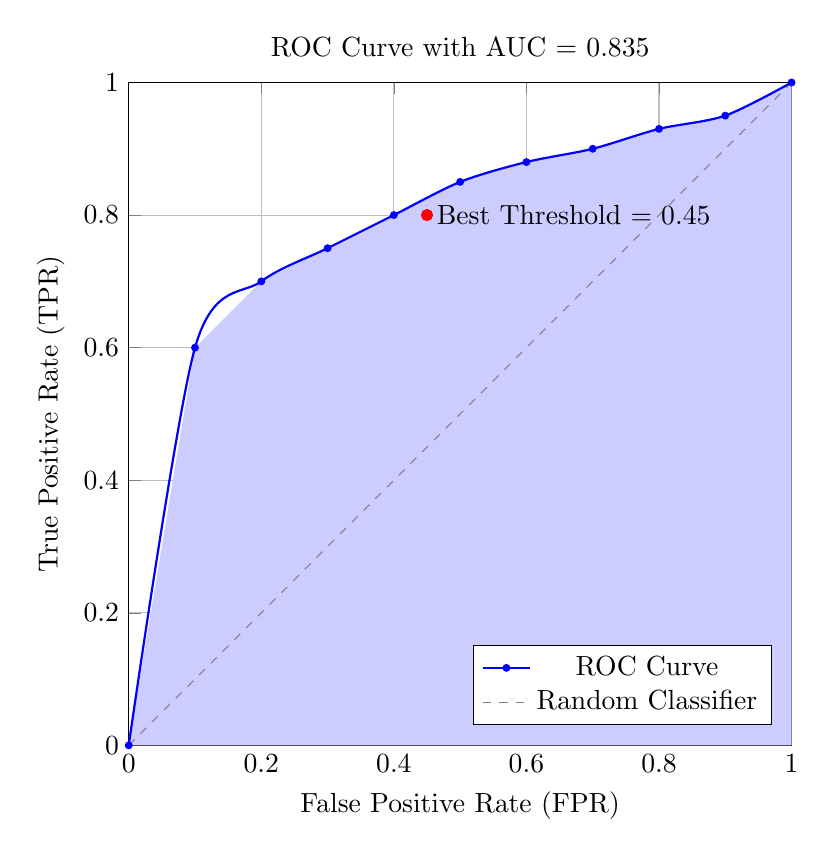
\begin{tikzpicture}
\begin{axis}[
    width=12cm,
    height=10cm,
    xlabel={False Positive Rate (FPR)},
    ylabel={True Positive Rate (TPR)},
    title={ROC Curve with AUC = 0.835},
    xmin=0, xmax=1,
    ymin=0, ymax=1,
    grid=major,
    axis equal image,
    legend pos=south east,
    enlargelimits=false,
    clip=false
]

% ROC curve sample points (replace with actual values if available)
\addplot [
    thick,
    blue,
    mark=*,
    mark options={scale=0.5},
    smooth
] coordinates {
    (0,0) (0.1,0.6) (0.2,0.7) (0.3,0.75) (0.4,0.8)
    (0.5,0.85) (0.6,0.88) (0.7,0.9) (0.8,0.93) (0.9,0.95) (1,1)
};
\addlegendentry{ROC Curve}

% Diagonal random line
\addplot[dashed, gray] coordinates {(0,0) (1,1)};
\addlegendentry{Random Classifier}

% AUC area shading
\addplot [
    name path=AUCtop,
    draw=none
] coordinates {
    (0,0) (0.1,0.6) (0.2,0.7) (0.3,0.75) (0.4,0.8)
    (0.5,0.85) (0.6,0.88) (0.7,0.9) (0.8,0.93) (0.9,0.95) (1,1)
};

\path[name path=AUCbase] (axis cs:0,0) -- (axis cs:1,0);

\addplot [
    blue!20
] fill between [
    of=AUCtop and AUCbase
];

% Best threshold annotation point
\addplot[only marks, red, mark=*, mark size=2pt] coordinates {(0.45,0.8)};
\node[anchor=west] at (axis cs:0.45,0.8) {Best Threshold = 0.45};

\end{axis}
\end{tikzpicture}

\end{document}